%************************************************
\chapter{Modeling Stochastic Dynamics of Active Matter}\label{ch:modelingActiveMatter}
%************************************************
In \autoref{ch:activeMotion} the importance and relevance of understanding migration, motion and search strategies in many different fields has been outlined. In order to understand and analyze such processes mathematical modelling is a commonly used tool. A broad field of possible modelling approaches is based on the so called \textit{Random Walk} and different extensions on it.

The random walk is a stochastic process that describes successive random steps on a mathematical space such as a hypothetical particle that walks on the integers $\mathbb{Z}$. The most basic version of the random walk is the \textit{\ac{SRW}}. It is unbiased (isotropic), meaning that the walker has no preference for one specific direction, and uncorrelated in direction, meaning that the history of previous steps' directions has no influence on the step direction at a given time.

More complex random walk versions build on the \acs{SRW} and extend it.

\section{The Simple Isotropic Random Walk}
Consider a one-dimensional lattice which is split into discrete sites as it is shown in \autoref{fig:1DSRW}. On this lattice, in each discrete timestep, a hypothetical particle (the \textit{walker}) is able to jump from its current site to the neighbouring sites, each with equal probabilities $p=1/2$. Therefore, the state of the walker can be described by the discrete time $n \in \mathbb{N}$ and position $m \in \mathbb{Z}$. Having the walker start at the origin ($m=0$), after one time step, it will either be at site $m=-1$ or $m=1$, each with probability $p=1/2$. After another time step, accordingly, the walker can be at sites $m=-2$ or $m=2$, each with probability $p=1/4$, or at the origin $m=0$ with probability $p=1/2$. In this manner one can continue in order to find the probabilities for being at each site at a given time.

\begin{figure}[bth]
 \myfloatalign
 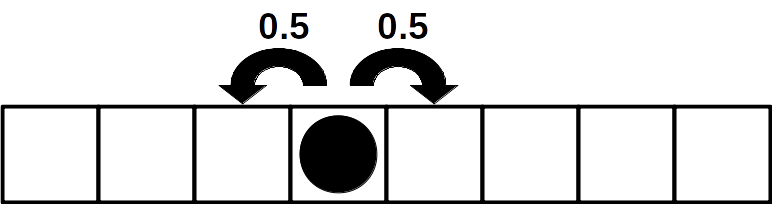
\includegraphics[width=0.8\linewidth]{gfx/1DSRW}
 \caption[\acs{SRW} on a one-dimensional lattice]{\acs{SRW} on a one-dimensional lattice. Black arrows indicate the possible sites in the next step with according probabilities.}\label{fig:1DSRW}
\end{figure}

Some important and useful quantities, however, are the mean position \mbox{$\mathbb{E}\left[M_n\right]$} and the \textit{\ac{MSD}} \mbox{$\mathbb{E}\left[M^2_n\right]$}, which are defined as
\begin{equation}
 %\label{eq:}
 \begin{aligned}
  \mathbb{E}\left[M_n\right]&=\sum^\infty_{m=-\infty}mp\left(m,n\right),
  \\
  \mathbb{E}\left[M^2_n\right]&=\sum^\infty_{m=-\infty}m^2p\left(m,n\right).
 \end{aligned}
\end{equation}
Here, $p\left(m,n\right)$ denotes the \textit{probability mass function}.

As the single steps of the walk are independent from each other, these quantities are easily derived. One obtains
\begin{equation*}
 \mathbb{E}\left[M_n\right]=0,
\end{equation*}
which illustrates the isotropy or absence of a bias, and
\begin{equation*}
 \mathbb{E}\left[M^2_n\right]=n,
\end{equation*}
the typical property of \textit{diffusion} (\acs{MSD} linear in time). Indeed, the \acs{SRW} is used to model diffusive motion \cite{codling:2008} and therefore cannot be used for active, directed motion. However, it is still a good starting point for extended models.

\section{The Biased Random Walk}
\graffito{The \acs{SRW} is a special case of the \acs{BRW} for $p=1/2$.}
By introducing a hopping probability $p \neq 1/2$ in the \acs{SRW} one obtains the \textit{\ac{BRW}}. The situation for the one-dimensional case is depicted in \autoref{fig:1DBRW}.

\begin{figure}[bth]
 \myfloatalign
 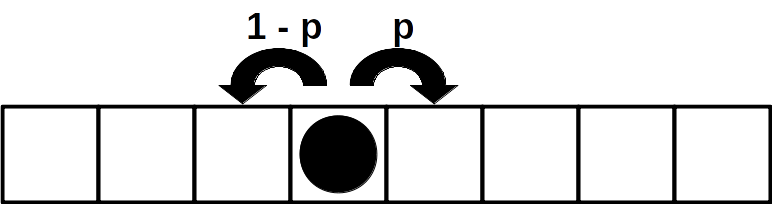
\includegraphics[width=0.8\linewidth]{gfx/1DBRW}
 \caption[\acs{BRW} on a one-dimensional lattice]{\acs{BRW} on a one-dimensional lattice. Black arrows indicate the possible sites in the next step with according probabilities.}\label{fig:1DBRW}
\end{figure}

Again one can easily derive the mean position and the \acs{MSD}. One obtains
\begin{equation*}
 \mathbb{E}\left[M_n\right]=n\left(2p-1\right),
\end{equation*}
which is nonzero (except for $p=1/2$) as a result of the introduced asymmetrical hopping rates. This drift to one side illustrates the walker's preference for one direction. For the \acs{MSD} one gets
\begin{equation*}
 \mathbb{E}\left[M^2_n\right]=4np\left(1-p\right)+n^2\left(4p^2-4p+1\right),
\end{equation*}
and thus \mbox{$\mathbb{E}\left[M^2_n\right]\propto n^2$}, which is typical for \textit{ballistic} motion. However, since the mean position drifts, in this case it is more meaningful to take a look at the dispersal about the mean position, which is defined as
\begin{equation}
 \sigma^2_n=\sum^\infty_{m=-\infty}\left(m-\mathbb{E}\left[M_n\right]\right)^2p\left(m,n\right).
\end{equation}
This quantity is easily obtainable as well and one derives
\begin{equation*}
 \sigma^2_n=4np\left(1-p\right).
\end{equation*}
This shows that the dispersal about the mean position is only linear in time and therefore the walker diffuses about its mean position. In other words: in its own rest frame the walker performs diffusive motion.

Because of its drift component the \acs{BRW} is a possible model to describe directed motion, however, it is only applicable under certain circumstances and given certain requirements, which will be explained later on. For now, one more random walk model will be introduced.

\section{The Persistent Random Walk}
So far the introduced random walk models have been uncorrelated and steps were independent from each other. In the \textit{\ac{PRW}} (or also \textit{\ac{CRW}}) this is not the case. Instead, at a given time the probabilities for the different directions of the next step are dependent on the direction of the very previous step. In other words: it matters from which direction the walker came from in the previous step, the walker has some kind of short memory.

The \acs{PRW} model defines a \textit{persistency} parameter $p \in \left[0,1\right]$ which gives the probability to keep going in the same direction. Therefore, in the one-dimensional case there are two possible ways of how a walker has reached its current side, leading to two possible scenarios of how it will continue its walk which are shown in \autoref{fig:1DPRW}.
\graffito{A \acs{PRW} with persistency parameter $p=1/2$ is equivalent to the \acs{SRW}.}

\begin{figure}[bth]
    \myfloatalign
    \subfloat[][Coming from the left site.]{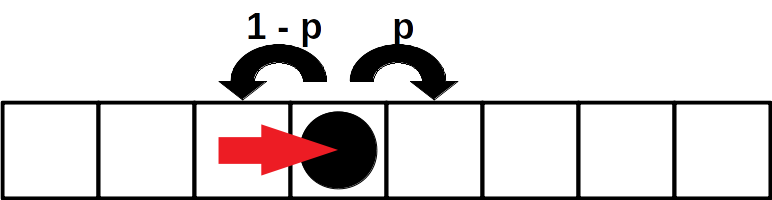
\includegraphics[width=.45\linewidth]{gfx/1DPRWfleft}} \quad
    \subfloat[][Coming from the right site.]{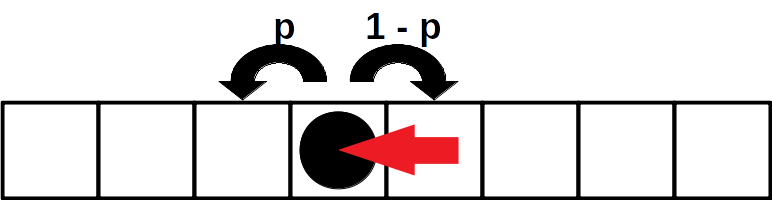
\includegraphics[width=.45\linewidth]{gfx/1DPRWfright}}
    \caption[\acs{PRW} on a one-dimensional lattice]{The two possible scenarios which can happen during the one-dimensional \acs{PRW}. Red arrows indicate the direction of movement in the previous step, black arrows indicate the possible sites in the next step with according probabilities.}\label{fig:1DPRW}
\end{figure}

Consequently, walks with $p < 0.5$ tend to reverse the direction of movement leading to \textit{anti-persistent motion}, while walks with $p > 0.5$ reinforce the direction of movement leading to \textit{persistent motion}. For the trivial cases of $p = 0$ the walker only jumps back and forth and for $p = 1$ it keeps going in one direction without ever reversing, which is a ballistic flight.

For the mean position and the \acs{MSD} one obtains \cite{shaebani:2014}
\begin{align*}
 \mathbb{E}\left[M_n\right] &= 0,
 \\
 \mathbb{E}\left[M^2_n\right] &= \frac{1+p}{1-p}n + \frac{2p}{\left(1-p\right)^2}\left(p^n-1\right).
\end{align*}

The result for the mean position is not surprising as there is no bias or preferred direction in the \acs{PRW}. However, the result for the \acs{MSD} is more interesting. Here one needs to differentiate between short and long term behavior.

For short times one derives
\begin{equation*}
 \mathbb{E}\left[M^2_n\right]\propto n^\alpha,
\end{equation*}
where $\alpha = 1+\ln\left(1+p\right)/\ln{2}$ \cite{shaebani:2014}. Considering only the non-trivial case of $p\in\left(0,1\right)$ gives $\alpha\in\left(1,2\right)$ and therefore the short term behavior is \textit{superdiffusive}.

For long times ($n\rightarrow \infty$) the second part of the right-hand side becomes a constant and the first part defines the behavior. This means that the \acs{MSD} is linear in time and the motion becomes diffusive.

Therefore, the \acs{PRW} shows a transition from superdiffusive to diffusive motion, which makes it a possible model to describe active, persistent motion. And indeed, later on, it will be the model of choice in order to study different aspects of motion. For this purpose, the model is extended to two dimensions and a model in continuous space is introduced.

\subsection{Two-dimensional lattice} \label{ssec:2d-lattice}
On a two-dimensional lattice the persistency parameter $p$ gives the probability to keep going in the same direction. However, instead of only one probability for the reversal of movement, there are two additional probabilites for turning to the right or left in respect to the direction of movement. To distinct between them, they will be denoted by $p_{\textrm{l}}$ and $p_{\textrm{r}}$, respectively. The probability of reversing the direction of motion is than computed by $p_{\textrm{b}} = 1 - p - p_{\textrm{l}} - p_{\textrm{r}}$. This means that for a walker at any given time there are four possible ways of how it has reached its current site and therefore there are four possible scenarios of how it will continue its walk which are shown in \autoref{fig:2DPRW}.

\begin{figure}[bth]
    \myfloatalign
    \subfloat[][Coming from the left site.]{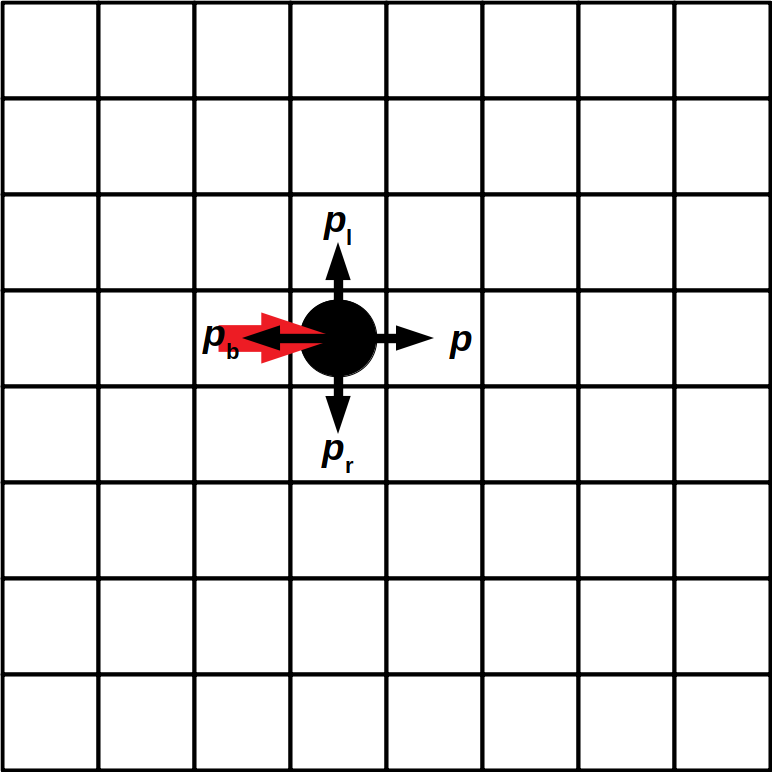
\includegraphics[width=.45\linewidth]{gfx/2DPRWfleft}} \quad
    \subfloat[][Coming from the right site.]{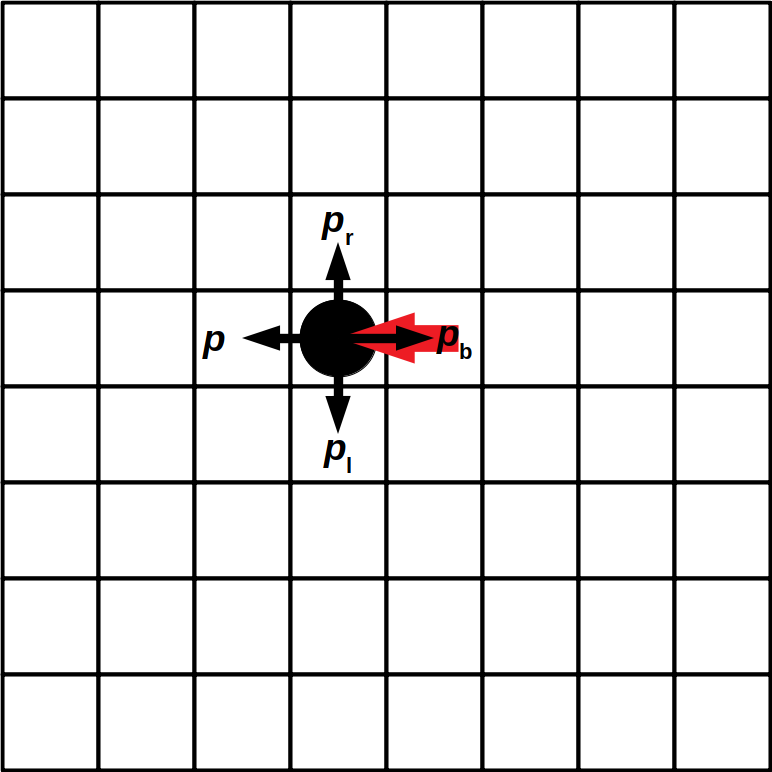
\includegraphics[width=.45\linewidth]{gfx/2DPRWfright}}
    \\
    \subfloat[][Coming from the upper site.]{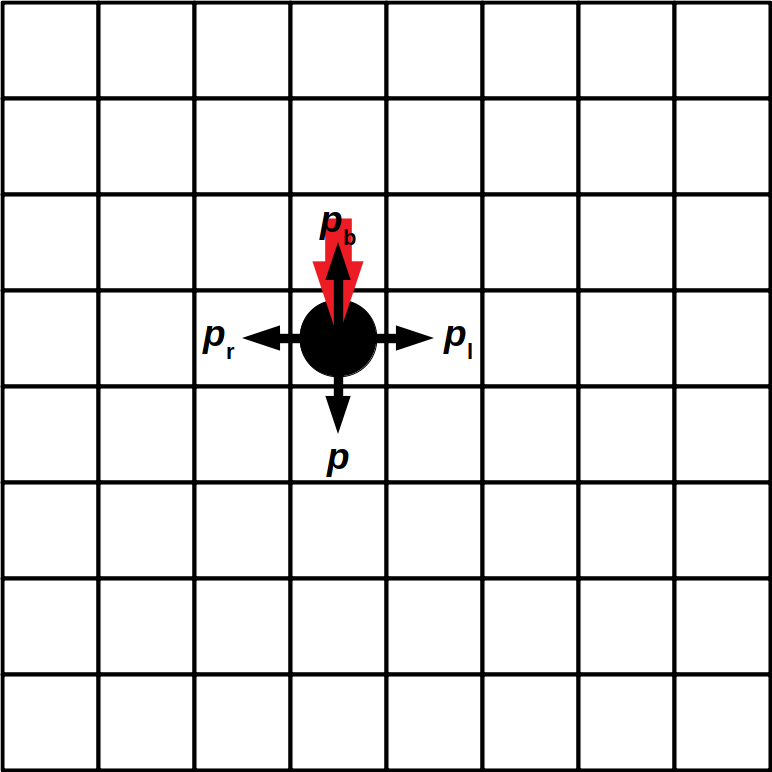
\includegraphics[width=.45\linewidth]{gfx/2DPRWftop}} \quad
    \subfloat[][Coming from the lower site.]{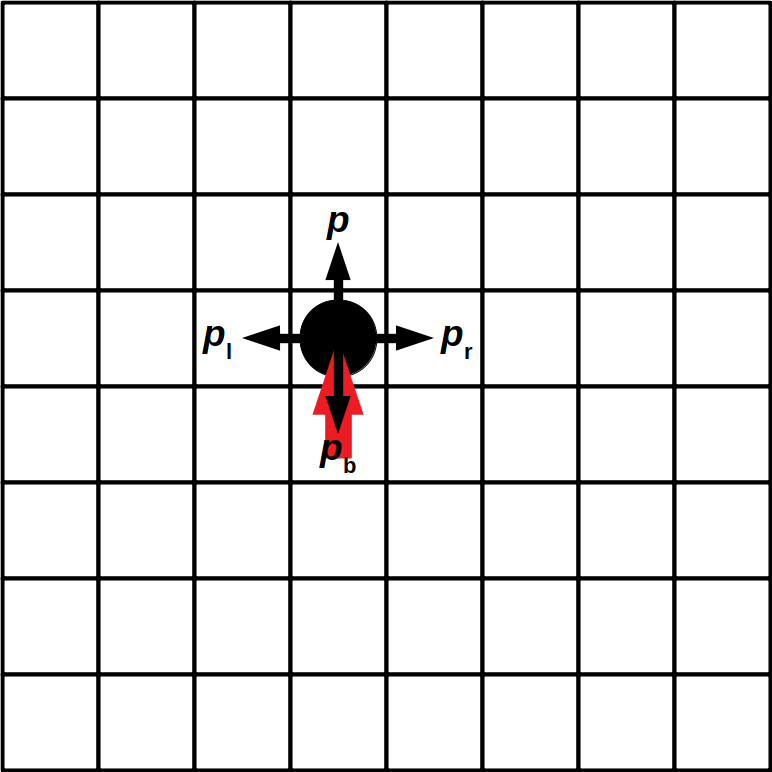
\includegraphics[width=.45\linewidth]{gfx/2DPRWfbot}}
    \caption[\acs{PRW} on a two-dimensional lattice]{The four possible scenarios which can happen during the \acs{PRW} on a two-dimensional lattice. Red arrows indicate the direction of movement in the previous step, black arrows indicate the possible sites in the next step with according probability.}\label{fig:2DPRW}
\end{figure}

Here, the analytical derivation of the mean position and the \acs{MSD} is much more complex than in the one-dimensional case and, since those quantities are not of much importance now, will be skipped. However, there are different other meaningful quantities that can be derived under certain simplifications, which will be explained below.

\subsection{Two-dimenional continuous space}
For the two-dimensional continuous \acs{PRW}, instead of hopping probailities, one needs a continuous turning angle distribution in order to determine the direction of movement. Additionally, the step-length can be chosen from a step-length distribution. Nevertheless, one can still define a persistency parameter.

Considering the turning angle distribution $R\left(\phi\right)$, one can define the mean cosine $c$ and mean sine $s$ of the turning angle as
\begin{equation}
 \label{eq:meanCosSin}
 \begin{aligned}
  c &= \mathbb{E}\left[\cos\left(\phi\right)\right] = \int\displaylimits^\pi_{-\pi} \cos\left(\phi\right)R\left(\phi\right)\textrm{d}\phi,
  \\
  s &= \mathbb{E}\left[\sin\left(\phi\right)\right] = \int\displaylimits^\pi_{-\pi} \sin\left(\phi\right)R\left(\phi\right)\textrm{d}\phi.
 \end{aligned}
\end{equation}
From these quantities one can extract information about the \acs{PRW}. The mean sine measures the relative probability of clockwise and anticlockwise turns. For most applications, however, the turning angle distributions are symmetric and, hence, the mean turning angle $\phi_{\textrm{mean}}$ as well as the mean sine $s$ are zero. In this case, the quantitiy $c$ is a measure of the correlation or persistency and therefore, the mean cosine $c$ as defined in \autoref{eq:meanCosSin} will be called persistency parameter $p$ hereinafter. Note that $p\in\left[-1,1\right]$ can be negative and depending on its value the motion is either anti-persistent, diffusive or persistent. An example distribution for each regime is shown in \autoref{fig:PRWTurningAngleDistribution}.

\begin{figure}[bth]
    \myfloatalign
    \subfloat[][Anti-persistent distribution with negative persistency parameter $p$.]{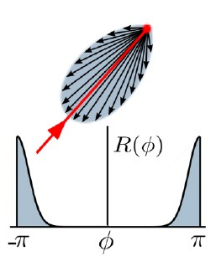
\includegraphics[width=.3\linewidth]{gfx/AntiPersTurnAngleDistri}} \quad
    \subfloat[][Diffusion distribution with persistency parameter $p=0$.]{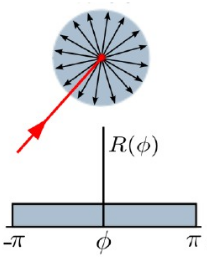
\includegraphics[width=.3\linewidth]{gfx/DiffTurnAngleDistri}} \quad
    \subfloat[][Persistent distribution with positive persistency parameter $p$.]{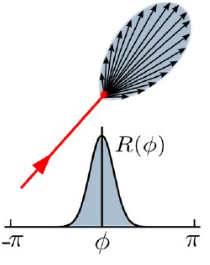
\includegraphics[width=.3\linewidth]{gfx/PersTurnAngleDistri}} 
    \caption[Turning angle distributions in the 2D \acs{PRW}]{Exemplary turning angle distributions and directions of movement in the context of the two-dimensional continuous \acs{PRW}. Red arrows indicate the direction of movement in the previous step, black arrows indicate possible directions of movement in the next step, with length being proportional to the probability. \cite{shaebani:2014}}\label{fig:PRWTurningAngleDistribution}
\end{figure}

%Now that these models and methods have been briefly introduced, the two-dimensional lattice model will be slightly modified and discussed in more detail.



%*****************************************
%*****************************************
%*****************************************
%*****************************************
%*****************************************
